% Thiyyyyyy was converted to LaTeX by Writer2LaTeX ver. 1.1.8
% see http://writer2latex.sourceforge.net for more info
\documentclass[review,letterpaper]{elsarticle}

\usepackage{array,supertabular}
\usepackage{color}
\usepackage{amsmath,amssymb,amsfonts}

\usepackage{graphicx,epstopdf}
%\usepackage{pstool}
\newcommand{\comment}[1]{} % use this line to hide the comments instead

\providecommand{\e}[1]{\times 10^{#1}}
% Outline numbering
\begin{document}



\begin{frontmatter}

\title{Propagators for the time-dependent Schr\"odinger equation in an adaptive, discontinuous, multi-wavelet basis}

\author[add]{Jun Jia}         \ead{jakiej@gmail.com}
\author[add]{Nicholas Vence}  \ead{nickvence@gmail.com}
\author[add]{Robert Harrison} \ead{harrisonrj@ornl.gov}
\author[add]{George Fann}     \ead{fanngi@ornl.gov}

\begin{abstract}

We present and compare explicit (high-order exponential) and implicit
(semi-group quadrature-collocation) propagators for the linear and non-linear time-dependent
Schr\"odinger equations within an adaptive, discontinuous, multi-wavelet basis in real space.
To control the non-physical frequencies present in the simulation, we use a bandlimited the free-space propagator.
The numerical results of a one-dimensional, linear test problem show that the gradient-corrected, exponential splitting requires fewer free-space convolutions than the quadrature-collocation method (QCM).
However, QCM has better control of the high-frequency noise, which is essential for efficient, high-dimension applications. The convergence behavior of the linear and non-linear problems are similar. Finally, we conclude with the propagation of an atomic system in an intense, attosecond laser pulse.
\end{abstract}

\begin{keyword}
Multi-wavelet; Multi-resolution analysis; Time Propagation; ab initio electron structure;
Green's function; time-dependent Schr\"odinger equation
\comment{
{\em Subject classifications:}
  65B05, % extrapolation to the limit, deferred corrections
  65F10, % Iterative methods for linear systems
  65M99. % New numerical methods for PDEs.
}
\end{keyword}

\end{frontmatter}



\section{Introduction}
Many physical applications require time-dependent solutions.
For instance, the complete treatment of molecular hydrogen in an intense, elliptically-polarized, infrared, laser pulse requires seven dimensions (7D): six to capture electron-electron correlation and one for the internuclear coordinate.
When a high-dimensional solution contains information on differing length scales, standard computational techniques are inadequate.
For example a 7-dimensional (7D), fixed-grid simulation with only 100 points/dimension, would require one of the largest, distributed-memory computers.
This resolution, however, is inadequate to describe an energetic electron driven far from the origin by the strong, infrared laser.
A multiresolution scheme, however, allocates scarce memory intelligently:
adaptively adding and removing basis functions.

Multiresolution analysis in a discontinuous, multi-wavelet bases is becoming a practical
approach for robust computation in many dimensions \cite{Alpert:1990,A-B-G-V:2002,ibmpaper,mrqc1}.
It provides the illusion of ``basis free'' science applications through the automatic,
adaptive refinement of its orthogonal basis.
This deep, local refinement enables a sparse representation
for functions containing information on a variety of length scales.
Finally, it guarantees finite precision offering a reasonable trade-off between
accuracy, efficiency, and ease of use.
While multiresolution analysis has been established for static \cite{mrqc1}
and dynamic \cite{Vence:2012iy} electron structure problems,
this paper describes the optimization of time evolution.

The adaptive refinement and truncation of the discontinuous, multi-wavelet basis complicates time evolution.
The discontinuities introduce non-physical, unbounded frequencies.
The Green's function of the time-dependent
Schr\"odinger equation (TDSE) has unbounded curvature (see \figurename~\ref{F:g0}-left),
which is impossible to represent in a finite-precision basis. A truncation in momentum space
bounds this curvature producing a band limited propagator: one that ignores frequencies above
the band limit in momentum space. While potentially truncating meaningful, high-energy events, the band limited
propagator has the benefit of filtering the high frequency noise inherent in the adaptive,
discontinuous, polynomial basis. Thus, we exchange the high-frequency dilemma for a trade-off
between efficiency (a low band limit) and accuracy (a high band limit).

The numerical requirements of multiresolution analysis limit our choice of time evolution methods.
Unitarity is required for stability; this eliminates the popular Lanczos method \cite{Leforestier:1991co}.
Low-order, implicit schemes are stable, but have an impracticably small time step.
Thus, we seek high-order propagators to enable larger time steps despite
the presence of high-frequencies.

We examine two complementary classes of propagators:
exponential splitting with gradient corrections and Quadrature Collocation Methods (QCM).
These propagators are applied to the linear and non-linear TDSE in one dimension (1D)
to determine their efficiency over a range of physical problems.
The Lippmann-Schwinger (or semi-group) form of the TDSE side steps many of the
high-frequency difficulties by relying upon the existence of an exponential for its linear part.

The paper is structured as follows. In Sec. \ref{S:freeProp} we review the free-space
propagator for the TDSE and formulate a bandwidth-limited version suitable for practical computation.
The accuracy of this propagator is demonstrated by comparing the numerical
evolution of a 1D Gaussian wave packet with its analytic result.
In Sec. \ref{S:prop}, we explore exponential propagators
and the QCM from the Lippmann-Schwinger (semi-group) form of the TDSE.
In Sec.~\ref{S:modelProblems} we define the model problems,
used for comparison in Sec.~\ref{S:Results}.
Finally, in Sec.~\ref{S:hatom} we examine an application
of Chin-Chen \cite{Chin:2001vs} propagating a 3D, atomic wave functions in an intense laser field.
This work is based on the framework for Multiresolution ADaptive Numerical
Environment for Scientific Simulation (MADNESS) \cite{madnessDOC}.
Atomic units (where Plank's constant $\hbar$, the charge and mass of an
electron are all set to unity) are used throughout this paper.




\section{Free-space propagator}
\label{S:freeProp}

\subsection{Theory}
The Hamiltonian operator $\hat{H} = T+V$ defines the behavior of a wave function
$\psi (x,t)$ in the TDSE:
\begin{equation}
\hat{H}\psi (x,t)=i\frac{\partial }{\partial t}\psi (x,t),
\label{E:tdse}
\end{equation}
where $T$ is the kinetic energy operator and $V$ is a given potential.
In free-space ($V=0$) the TDSE becomes
\begin{equation}
i\dot{\psi } = T \psi = -{\frac{1}{2}}\nabla ^{2}\psi .
\end{equation}
The real-space kernel of the free-space propagator for this Schr\"odinger equation is
\begin{equation}
G_{0}(x,t)=\frac{1}{\sqrt{2\pi it}}e^{-{\frac{x^{2}}{2it}}}.
\end{equation}
Since the energy dependent phase is an important part of the solution, it is worth
examining the effect of this operator on a plane wave corresponding to a beam of
particles with velocity $v$:
\begin{equation}
G_{0}(x,t)\ast e^{ixv}=e^{ixv-iv^{2}t/2}.
\end{equation}
This reminds us that the time dependence of a stationary state $e^{ivx}$, being an
eigenfunction of the kinetic energy operator, is entirely contained in a complex phase;
thus, the free-space propagator does not couple different spatial frequencies. This
exponential function reappears in Section \ref{S:linearTDSE} as the Galilean
translation factor.


\subsection{Band limiting}
The unbounded spectrum of $G_0$ in \figurename~\ref{F:g0}(a) makes a finite-precision representation impossible.
However, we are not interested in representing the full operator, only the components necessary
for the propagation of a band limited wave function. This is analogous to the upper energy
limit on a uniform grid. The band limit is applied by transforming $G_0$ to momentum
space, multiplying by a band limiting filter, and transforming back to real space.
The band limited $G_0$ is bounded both in real space [see \figurename~\ref{F:g0}(b)] and momentum space.

Consider the exact representation of the propagator in Fourier space:
\begin{equation}
{\hat{G}}_{0}(k,t)=e^{-i k^2t/2}.
\end{equation}
We band limit by applying a filter $F(k/c)$ that smoothly switches from zero to unity at $k=c$.
At present, we use a 30\textsuperscript{th}-order Butterworth filter (see inset in \figurename~\ref{F:g0})
\begin{equation}\label{seq:refText5}
F(\frac k c)=\left(1+\bigg(\frac{k}{c}\bigg)^{30}\right)^{-1}
\end{equation}
that is applied separately in each dimension to preserve the separability
of the resulting kernel.

The error incurred after a single application of the band limited $G_0$ deviates from unity by about $-{(\frac k c})^{30}$ for $k \ll c$.
Thus, if we desire frequencies up to a target band limit ($c_{target}$) with a precision
$\epsilon$ after  $N$ applications of the operator, then we should choose the actual band limit in
the filter such that $N(c_{target}/c)^{30}\le \epsilon$, that is $c\ge c_{target}(N/\epsilon )^{1/30}$.

Consider a calculation where we desire an accuracy of $\epsilon = 10^{-3}$ after $N = 10^5$ time steps.
To preserve the integrity of highest frequencies, which are most sensitive to error, we would choose
$c\ge 1.85c_{target}$. Similarly, for  $k\gg c$ the filter  $F(\frac k c)$ differs from zero by about  $(\frac k c)^{-30}$;
therefore the internal numerical approximation of the operator must include frequencies
 $2.15\times$ for a precision $10^{-10}$ and $2.5\times$ for a precision of $10^{-12}$.

\begin{figure}[ht]
\centering
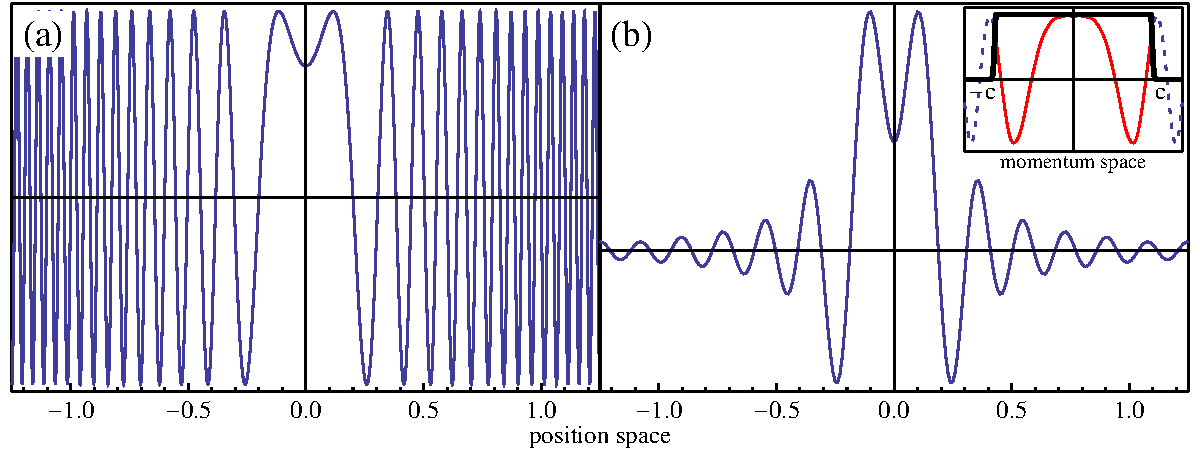
\includegraphics[width=4.5in]{freePP}
%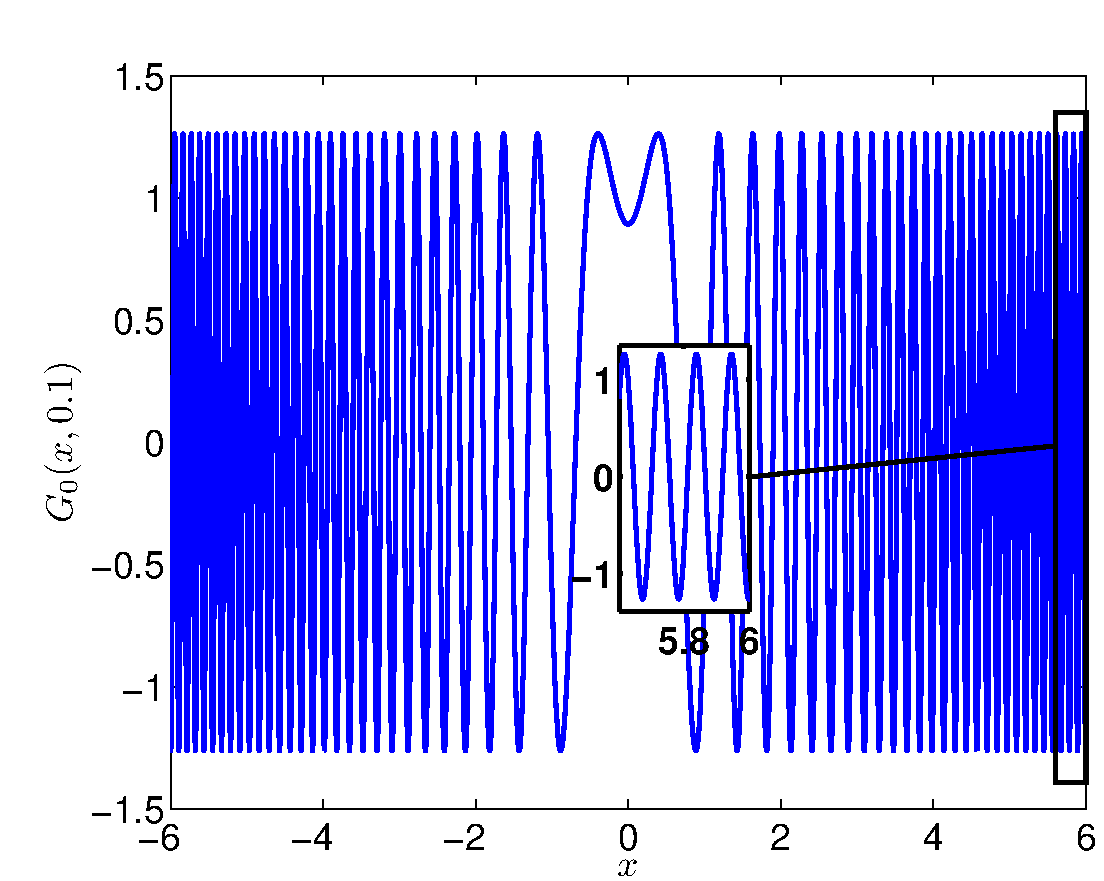
\includegraphics[width=2.2in]{g0}
%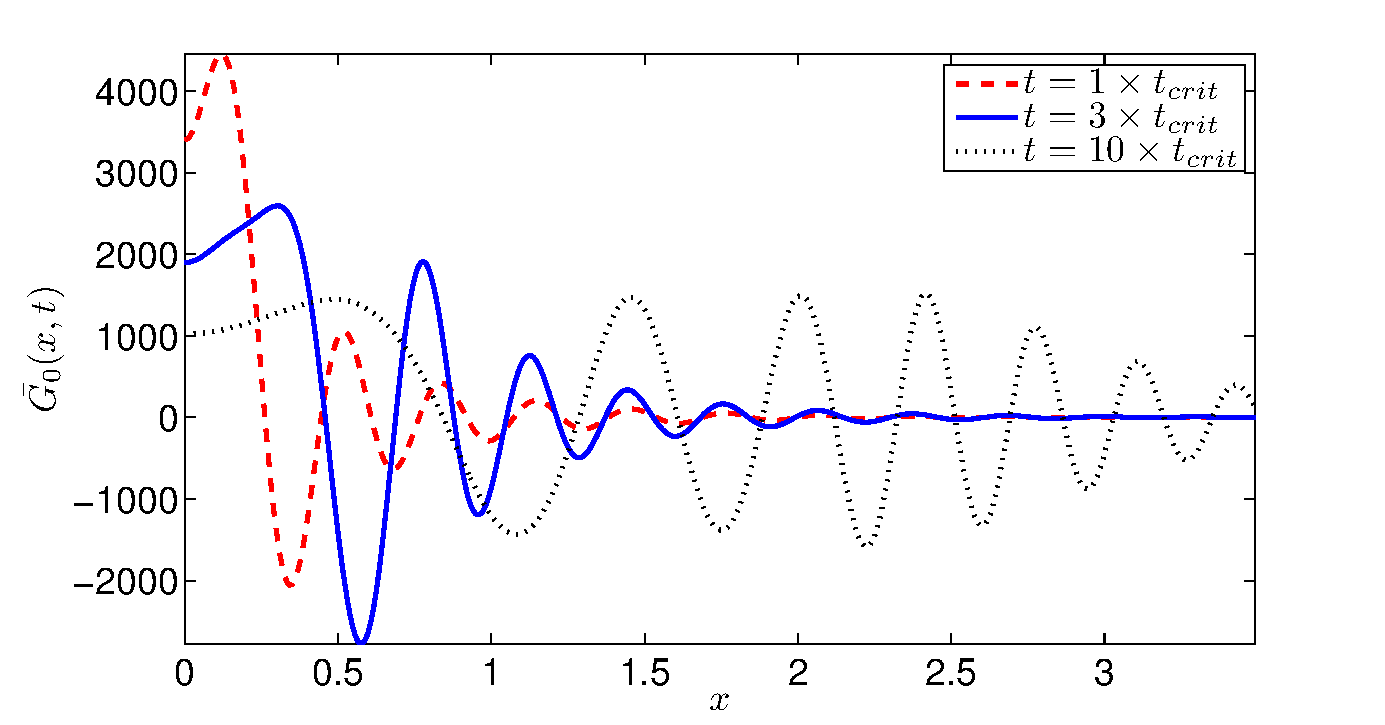
\includegraphics[width=2.2in,height=1.7in]{bandlimited}
\caption{(a) The real component of the 1D free particle propagator and (b) its band-limited counterpart. The band-limit (inset) in momentum space is the black line and the excluded Fourier components of the original function are dashed. }
\label{F:g0}
\end{figure}

While this operator is unconditionally stable and effectively unitary for frequencies below the
band limit  $c_{target}$, the cost of applying the operator grows rapidly when the time step exceeds
a critical value
\begin{equation}
t_{crit}=\frac{2\pi }{c^{2}}.
\end{equation}
This is due to the number of oscillations in the increased range of the real-space kernel
(see \figurename~\ref{F:g0}-right).

The discontinuous, spectral element basis is a computationally convenient
alternative to the finite element or finite difference methods.
Continuity emerges (within finite precision) with the application
of an appropriately constructed integral or differential operator \cite{Alpert:2002cx},
as is the case with the stencils used in finite difference methods.
Nevertheless, the adaptive, discontinuous, polynomial basis unavoidably
includes numerical, high-frequency components even when representing
smooth functions, and it is the insensitivity of the band limited $G_0$ to this
numerical noise that preserves the integrity of the wave function.



\subsection{The Real-space (scaling function) algorithm}
\label{S:bandLimitedProp}

At the coarsest level (n=0), a function is represented by a linear combination of scaling functions
\begin{equation}
\phi _{p}(x)=\left\{\begin{matrix}\sqrt{2p+1}P_{p}(2x-1)&0\le x\le 1\\0&\textrm{otherwise.}\end{matrix}\right.
\end{equation}
where $P_p(x)$ are the Legendre polynomials.
These parent scaling functions (n=0) are shifted and dilated as the representation of the function is refined.
\begin{align}
\phi^{n \ell}_p(x) = 2^{n/2} \phi_p(2^n x-\ell)
\end{align}

An exact application of the free-space propagator (in the scaling function basis)
doubles the number of required basis functions, i.e.,
\begin{equation}
\label{E:matElem}
r_{p}^{nl}=\int G_{0}(x)\phi _{p}^{nl}(x)dx=2^\frac n2\int G_{0}(x)\phi _{p}(2^{n}x-l)dx.
\end{equation}
The  $r_{p}^{nl}$ are combined with the pre-computed coefficients over the autocorrelation functions of the scaling function basis, as described in the appendix of \cite{mrqc1}.
In the real-space, the application of the kernel is a straightforward recombination
of the scaling function basis.  However, the application cost scales unfavorably
in a higher dimension simulation.  The scaling is improved by taking advantage
of the separability of the kernel $G_0$; that is, by successively applying the $1D$ $G_0$ in each dimension.

\figurename~\ref{F:freeSpace} demonstrates the effectiveness of the band limited, free-space propagator
by evolving a gaussian wave packet from $t = 0$ (left column) to $t = 100$ (right column) with $dt=10t_{crit}\approx0.15$.
The first (second) row shows the real (imaginary) part of the wave function being translated
from a simple, localized function to a highly oscillatory pattern; nevertheless, when recombined,
these components reproduce a smooth gaussian wave packet with bounded error (see \figurename~\ref{F:errorT100}).

\begin{figure}[hbtp]
\hspace{-.6in}
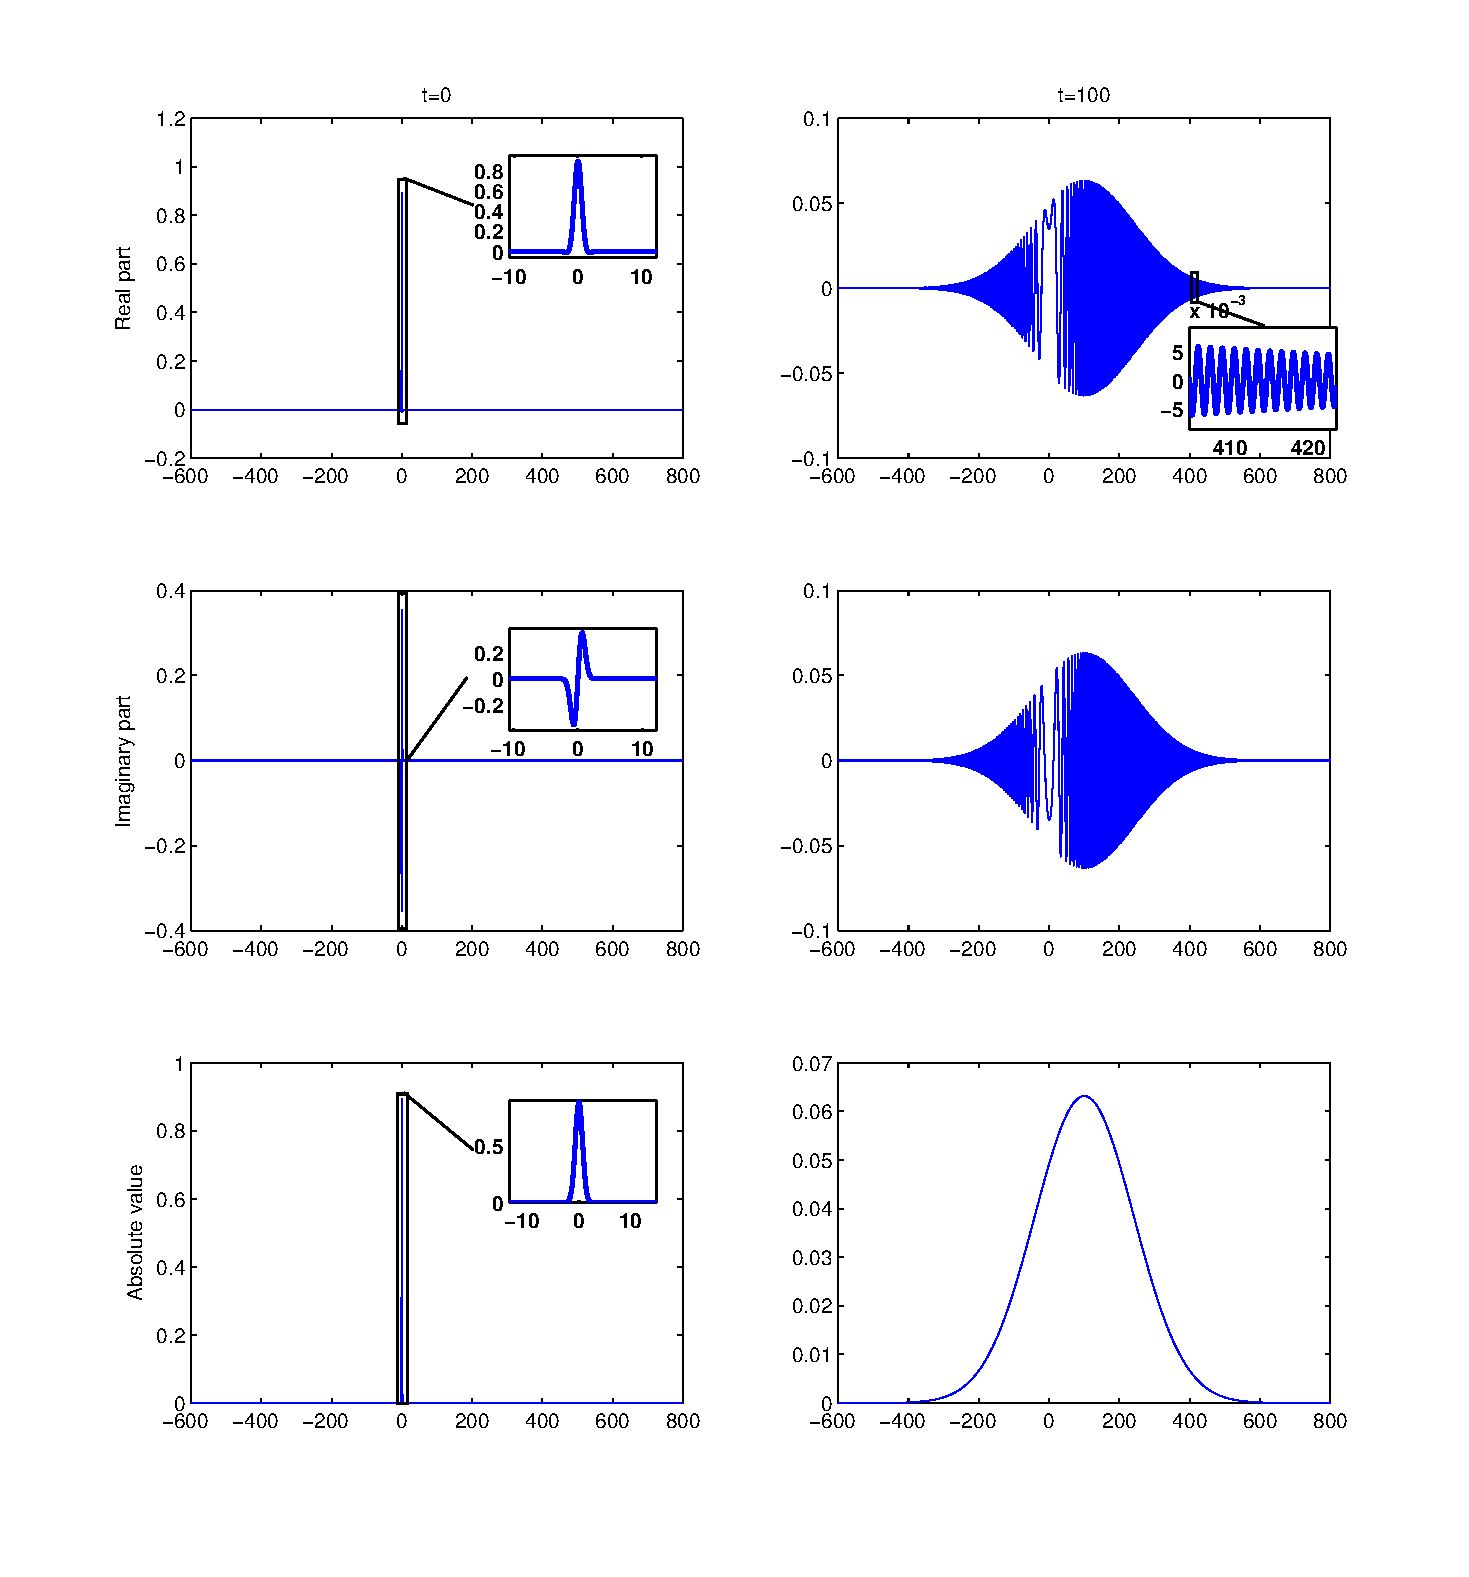
\includegraphics[width=5.6in,height=7in]{freeSpace}
\vspace{-.8in}
\caption{A 1D wave function (magnified in the insets) plotted over the spatial domain [-600, 800]
  before (left column at $t=0$) and after (right column at $t=100$) demonstrates
  the accuracy of band limited propagation (with $dt=10t_{crit}\approx0.15$). 
  The oscillatory  real (top row) and imaginary (middle) components preserve the Gaussian
  in the absolute value (bottom).}
\label{F:freeSpace}
\end{figure}

\begin{figure}[hbt]
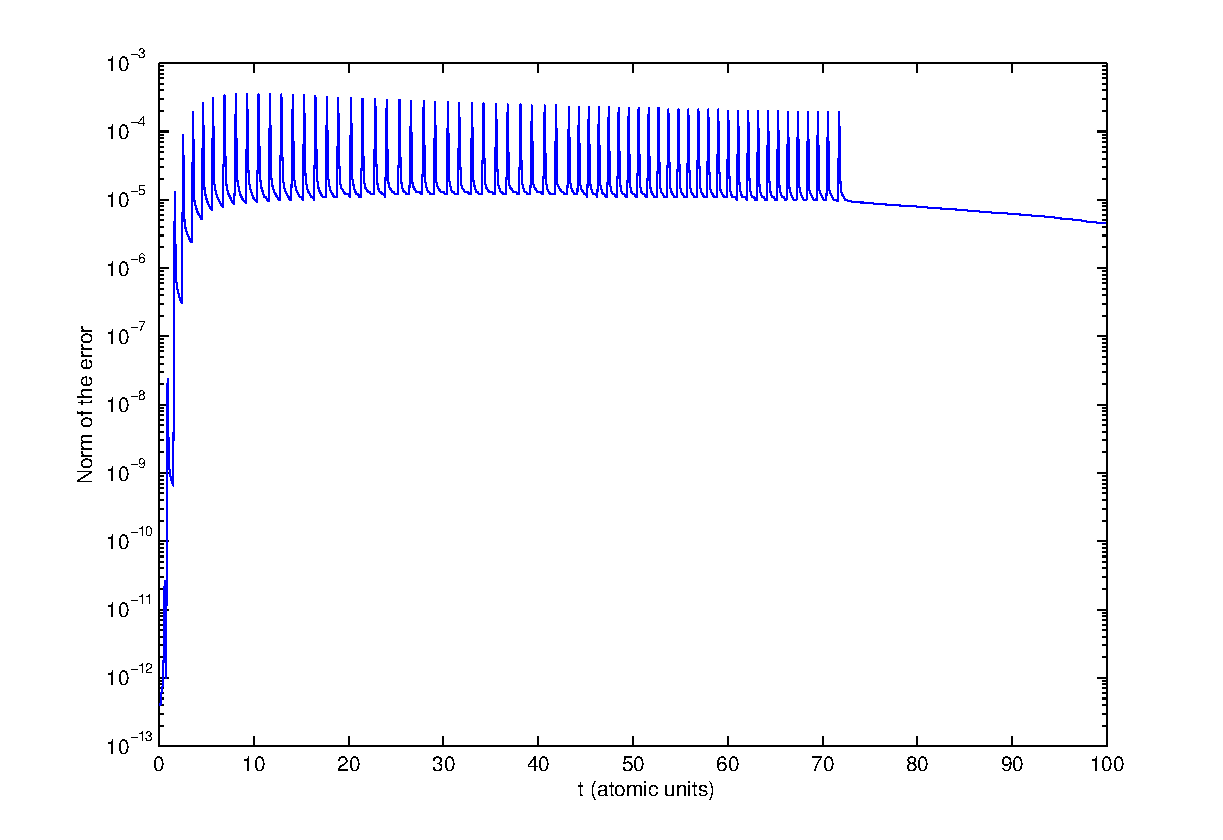
\includegraphics[width=5in]{errorT100}
\caption{The error of the wave function norm (see Fig. \ref{F:freeSpace}) during band limited propagation.}
\label{F:errorT100}
\end{figure}




\section{Propagators}
\label{S:prop}
\subsection{Exponential propagators}
\label{S:ExpProp}
Exponential propagators (see  \cite{Ta07} for a more complete introduction)
are unitary and symplectic. Since high order, exponential propagators allow longer time steps,
we examine several different time splitting schemes.

The popular Trotter propagator
\begin{equation}
\label{E:CC}
\mathcal{U}_{trot}(t+\tau,t) =
                     e^{-\frac{i \tau}2 T}
                     e^{-i {V}\tau}
                     e^{-\frac{i \tau}2 T}
                   + O\big(\tau^3 \big)
\end{equation}
is second order accurate with $e^{-\frac{i\tau}{2} T}$ representing an application of the free particle propagator.
Chin and Chen \cite{Chin:2001vs} derived a high-order propagator (CC)
\begin{eqnarray*}
\mathcal{U}_{cc}(t+\tau,t) &=&
e^{-{\frac{i t }{6}}V(t+\tau )}
e^{-{\frac{i\tau }{2}}{T}}
e^{-{\frac{2i\tau }{3}}\tilde{V}(t+\frac{\tau }{2})}
e^{-{\frac{i\tau }{2}}{T}}
e^{-{\frac{i\tau }{6}}V(t)}
+O(\tau^5) \notag\\
\tilde{V}(t)&=&V(t) - \tau^2 \alpha \left(\nabla V\right)^{2} \\
\alpha \left(\nabla V\right)^{2} &=& \frac{1}{48} [V,[T,V]] \notag
\end{eqnarray*}
that is accurate through fourth order in time; it does not require negative intermediate
time steps and is only slightly more expensive to apply than the second-order
accurate Trotter splitting.

Arbitrary, high-order exponential integrators can be constructed using the
force gradient algorithms \cite{force-gradient}. We examine the updating schemes for the optimal fourth- and sixth- order force gradient methods.
\newcommand{\VTV}{C}
Letting $C$ denote $(\nabla V)^2$, the forth-order exponential propagator (EP4) is
%\newcommand{\VTV}{C}{[V,[T,V]]}
\begin{equation}
\mathcal{U}_{4}(t+\tau,t) +O(\tau^5)=
e^{V \lambda \tau+\xi \VTV \tau^3}
e^{T \frac\tau 2}
e^{V(1-2\lambda)\tau+\chi \VTV \tau^3}
e^{T \frac\tau 2}
e^{V \lambda \tau+\xi \VTV \tau^3}
\end{equation}
with
\begin{equation}
\lambda=\frac16, \quad \xi=-\frac{17}{18000}, \quad \chi=\frac{71}{4500} .
\end{equation}
The sixth-order force-gradient method (EP6) is
\begin{eqnarray}
\mathcal{U}_{6}(t+\tau,t) +O(\tau^7)= \notag\\
e^{T \rho \tau} e^{V \nu \tau +\mu\VTV\tau^3} e^{T \theta \tau} e^{T (1-2(\theta+\rho)\frac \tau 2}\notag\\
e^{V(1-2(\lambda+\nu))\tau +\chi \VTV \tau^3}\notag\\
e^{T (1-2(\theta+\rho)\frac \tau 2} e^{T \theta \tau}e^{V \nu \tau +\mu\VTV\tau^3}e^{T \rho \tau}
\end{eqnarray}
with
\begin{eqnarray}
    \rho &=& 0.1097059723948682\notag\\
    \theta &=& 0.4140632267310831\notag\\
    \nu &=& 0.2693315848935301\notag\\
    \lambda &=& 1.131980348651556\notag\\
    \chi &=& -0.01324638643416052\notag\\
    \mu &=&  0.8642161339706166 \times {10}^{-3} .
\end{eqnarray}


\subsection{Quadrature Collocation Methods}
\label{S:QCM}
One of the main contributions of this paper is the analysis of the Quadrature Collocation Method
(QCM), which is based on the Lippmann-Schwinger equation or integral form of the TDSE:
\begin{equation}
\label{seq:refText13}
\psi (x,t)=\int dx'G_{0}(x-x',t)\psi (x,0)-i\int _{0}^{t}dt'\int dx'G_{0}(x-x',t-t')V(x',t')\psi (x',t').
\end{equation}
We approximate the time integral by
numerical quadrature using a polynomial expansion to capture the time dependence of the wave function.

We define  $p_{\mu }$ and  $\omega _{\mu }$ (for  $\mu =1,..,n$) to be the set of Gauss-Legendre  quadrature points and
weights on the interval  $t\in[0,1]$, and  $l_{\mu }(t)$ to be the Lagrange interpolating
polynomials of degree  $n$ that interpolates over the quadrature points.
The index  $\mu =0$ refers to  $t=0$.  The interpolating polynomial for the wave function is then

\begin{equation}\label{seq:refText14}
\bar{\psi }(t)=\sum _{\mu =0}^{n}\psi _{\mu }l_{\mu }(t/\tau )
\end{equation}
where for clarity we have hidden the  $x$-dependence and defined  $t_{\mu }=\tau p_{\mu }$
and  $\psi _{\mu }=\psi (x,t_{\mu })$.
Hiding the  $x$-dependence and using  $\text{*}$ to denote convolution over  $x$,
Eq.~\ref{seq:refText13} is approximated as
\begin{equation}\label{seq:refText15}
\psi (t)=G_{0}(t)\ast \psi _{0}-it\sum _{\nu =1}^{n}\omega _{\nu }G_{0}(t(1-p_{\nu }))\ast V(tp_{\nu })\psi (tp_{\nu }).
\end{equation}
which reduces to
\begin{equation}\label{seq:refText16}
\psi (\tau )=G_{0}(\tau )\ast \psi _{0}-i\tau \sum _{\mu =1}^{n}\omega _{\mu }G_{0}(\tau -t_{\mu })\ast V(t_{\mu })\bar{\psi }_{\mu }
\end{equation}
upon evaluation at $t=\tau$. Nevertheless, we must first obtain the wave function at the
intermediate times (indexed by  $\mu$).
To this end, we insert the polynomial approximation from Eq.~\ref{seq:refText15}
into Eq.~\ref{seq:refText16} and evaluate the integral at each  $t_{\mu }$
(defining for clarity  $t_{\mu \nu }=t_{\mu }p_{\nu }=\tau p_{\mu }p_{\nu }$)

\begin{equation}\label{qcform}
\psi _{\mu }=G_{0}(t_{\mu })\ast \psi _{0}-it_{\mu }\sum _{\nu =1}^{n}\omega _{\nu }G_{0}(t_{\mu }-t_{\mu \nu })\ast V(t_{\mu \nu })\bar{\psi }(t_{\mu \nu })
\end{equation}
This reduces to an  $n\times n$ system of equations whose solution is the $\psi _{\mu }$.
Finally, the sum in Eq.~\ref{seq:refText16} is evaluated to obtain  $\psi (\tau )$ which is
numerically described to be accurate $O(\tau ^{2n})$.

To assist the reader in the practical implementation of these methods we explicitly write the
equations for one and two Gauss-Legendre quadrature points.

\textit{One-point:} The quadrature point and weight are  $p_{1}=1/2,\: \omega _{1}=1$.
The interpolating polynomial is  $\bar{\psi }(t)=\psi _{0}+\frac{2t}{\tau }(\psi _{1}-\psi _{0})$
with its relevant values being  $\bar{\psi }(0)=\psi _{0}$,
$\bar{\psi }(\tau /4)=(\psi _{0}+\psi _{1})/2$, and  $\bar{\psi }(\tau /2)=\psi _{1}$.
The equation for the wave function at the quadrature point is

\begin{equation}
\bar{\psi }(\tau /2)=\psi _{1}=G_{0}(\tau /2)\ast \psi _{0}-\frac{i\tau }{4}G(\tau /4)\ast V(\tau /4)(\psi _{0}+\psi _{1})
\end{equation}
For sufficiently small  $\tau $ this will converge as a fixed-point iteration from the initial guess
$\psi _{1}=\psi _{0}$. The value of the wave function at the new time step is computed from

\begin{equation}
\psi (\tau )=G_{0}(\tau )\ast \psi _{0}-\frac{i\tau }{2}G(\tau /2)\ast V(\tau /2)\psi _{1}
\end{equation}



\textit{Two-points:} The quadrature points and weights are  $p_{1}=(1-1/\sqrt{3})/2$,
$p_{2}=(1+1/\sqrt{3})/2$, and  $\omega _{1}=\omega _{2}=1/2$. The quadratic interpolating
polynomials for the two quadrature points and zero are

\begin{equation}
\begin{matrix}l_{0}(s)&\text{=}&6(s-p_{1})(s-p_{2})\hfill\null \\l_{1}(s)&\text{=}&\frac{18s(s-p_{1})}{(3+\sqrt{3})\sqrt{3}}\hfill\null \\l_{2}(s)&\text{=}&\frac{18s(s-p_{2})}{(3+\sqrt{3})\sqrt{3}}\hfill\null \end{matrix}
\end{equation}
and the interpolating polynomial  $\bar{\psi }(t)$ is given by (15). The equations for the wave function at the quadrature points ( $t_{1}=\tau p_{1}$ and  $t_{2}=\tau p_{2}$) are then

\begin{equation}
\begin{gathered}\psi _{1}=G_{0}(t_{1})\ast \psi _{0}-it_{1}\left(G(t_{1}-t_{11})\ast V(t_{11})\bar{\psi }(t_{11})+G(t_{1}-t_{12})\ast V(t_{12})\bar{\psi }(t_{12})\right)\\\psi _{2}=G_{0}(t_{2})\ast \psi _{0}-it_{2}\left(G(t_{2}-t_{21})\ast V(t_{21})\bar{\psi }(t_{21})+G(t_{2}-t_{22})\ast V(t_{22})\bar{\psi }(t_{22})\right)\end{gathered}
\end{equation}



\section{Model Problems}
\label{S:modelProblems}
To compare the numerical behavior of the propagators mentioned in Section \ref{S:prop}, we time evolve
the ground state wave function for a model, 1D atom translating at a constant velocity  $v$.
Then, we explore a nonlinear variation by introducing an interaction potential in a second problem.

\subsection{The linear TDSE}
\label{S:linearTDSE}
We choose a numerically demanding problem that has an exact solution and is representative
of many physical applications (e.g. Section~\ref{S:hatom}).
The time-independent Hamiltonian
\begin{equation}
\hat{h}=-{\frac{1}{2}}\nabla ^{2}+V(x)
\end{equation}
has eigenfunctions $\phi (x)$
\begin{equation}
\hat{h}\phi(x) = E\phi (x) .
\end{equation}
The time-dependent Hamiltonian
\begin{equation}
\begin{gathered}
\hat{H}=-{\frac{1}{2}}\nabla ^{2}+V(x-vt)\\\hat{H}\psi (x,t)=E\psi (x,t)
\end{gathered}
\end{equation}
has similar eigenfunctions
\begin{equation}
\psi (x,t)=\phi (x-vt)e^{-i(E+v^{2}/2)t+ixv},
\end{equation}
these analytic functions are used to verify the accuracy of our simulations.
To facilitate an accurate, numerical solution, we choose a band limited potential
\begin{equation}
V(x)=-8e^{-x^{2}}
\end{equation}
with both discrete and continuum spectra.
We computed a high-accuracy solution of the time-independent problem
in Maple yielding the ground state energy calculated to machine precision:
$E_{0}=-6.188788775728797$.
The time-dependent problem was solved on a [-100,100] spatial domain with the atom initially
located at  $x=-90$ having a velocity  $v=3$.
Sixty time steps translated the peak of the wave packet from -90 to +90.


\subsection{The non-linear TDSE}
\label{S:nonLinearTDSE}
Now consider the previous Hamiltonian with \emph{two} particles having an interaction potential  $U(x_1 - x_2)$
\begin{equation}
\left(\hat{H}_1+\hat{H}_2+U(x_{1}-x_{2})\right)\Psi (x_{1,}x_{2,}t)=i\dot{\Psi }(x_{1,}x_{2,}t)
\end{equation}
where we assume the separability ansatz
\begin{equation}
\Psi (x_{1,}x_{2,}t)=\phi (x_{1,}t)\phi (x_{2,}t)
\end{equation}
which is the mean-field or Hartree approximation.
This requirement yields a one-particle state equation
\begin{gather}
\left(\hat{H}+u(x,t)\right)\psi (x,t)=i\dot{\psi}(x,t) \\
u(x,t) =\int U(x-x'){\left|{\phi (x',t)}\right|}^{2}dx'
\end{gather}
If  $U$ were the Coulomb potential, this would correspond to the mean electrostatic potential between
the two particles; however, we choose a local potential
\begin{equation}
U(x-x')=\delta (x-x')
\end{equation}
yielding the following non-linear equation
\begin{equation}
\left(\hat{H}+{\left|{\phi (x,t)}\right|}^{2}\right)\phi (x,t)=i\dot{\phi}(x,t).
\end{equation}
Using the same method in Section~\ref{S:linearTDSE},
we compute a high-accuracy solution with a ground state energy
of -5.497447807610323 repeating the same tests.




\section{Results}
\label{S:Results}
To compare the numerical behavior of the various propagators, we time evolve
the ground state wave function for a model, 1D atom translating at a constant velocity  $v$.
First, we explore the convergence of the error in the linear TDSE as a function of the step size ($dt$).
Then, we examine the refinement level and number of coefficients as a function of time.
Finally, we summarize the results of the nonlinear TDSE.

\subsection{Convergence: error vs step size}
We compare propagators using the linear TDSE as described in Section \ref{S:linearTDSE}.
Unless otherwise stated, a propagator's slope is taken from the middle line segment.
\begin{figure}[ht]
\centering
%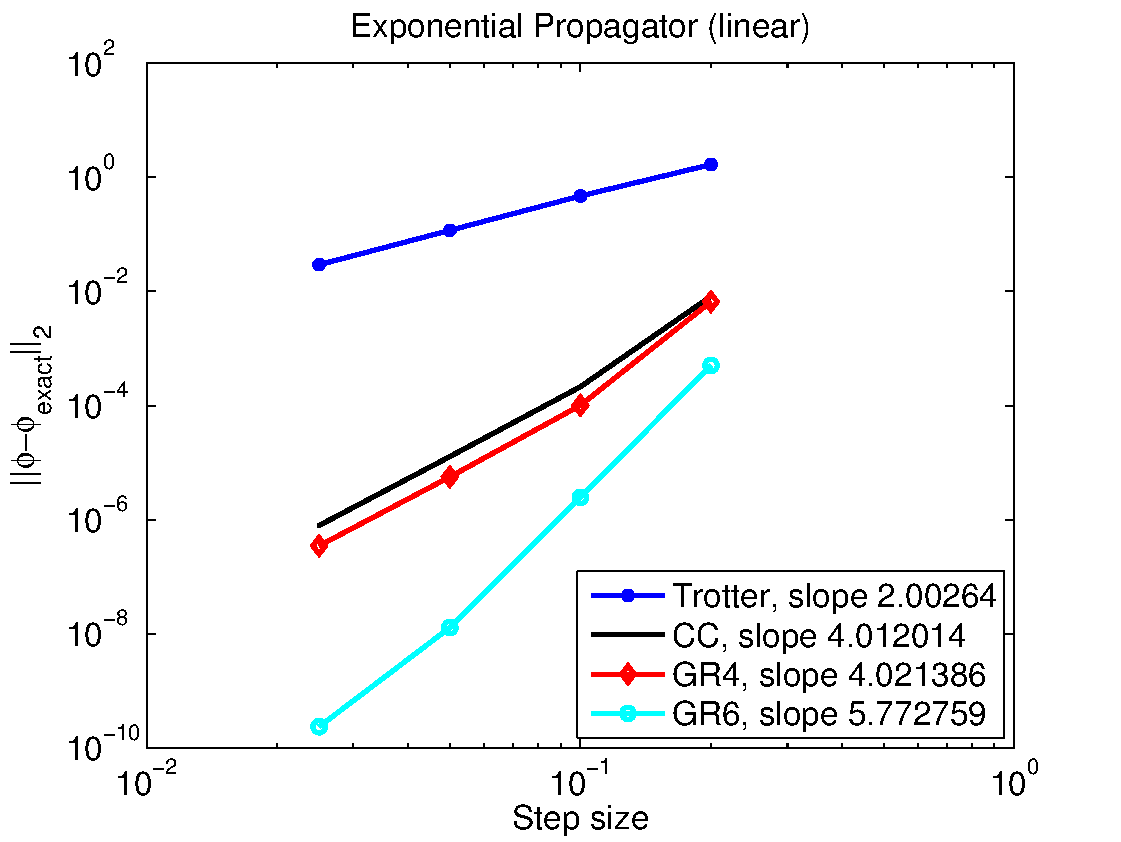
\includegraphics[width=5in,height=3.5252in]{error-norm-2}
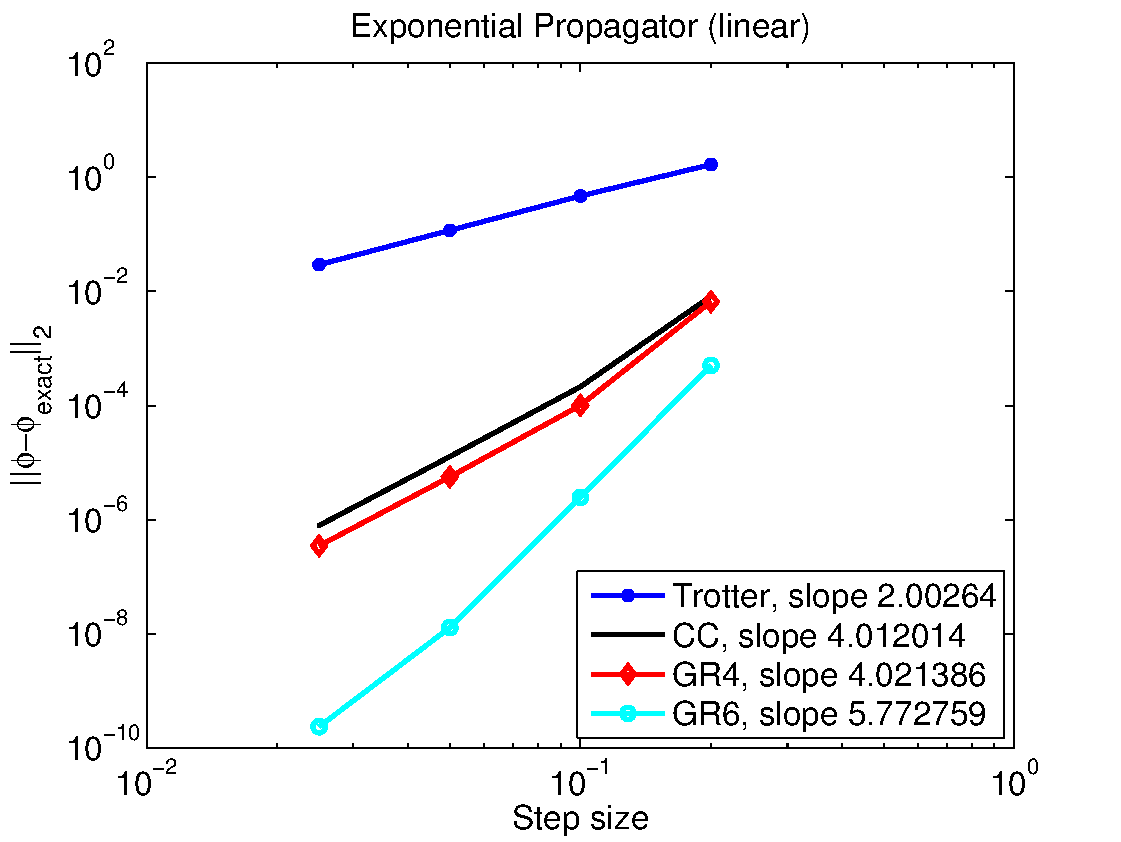
\includegraphics[height=1.7in]{error-norm-2}
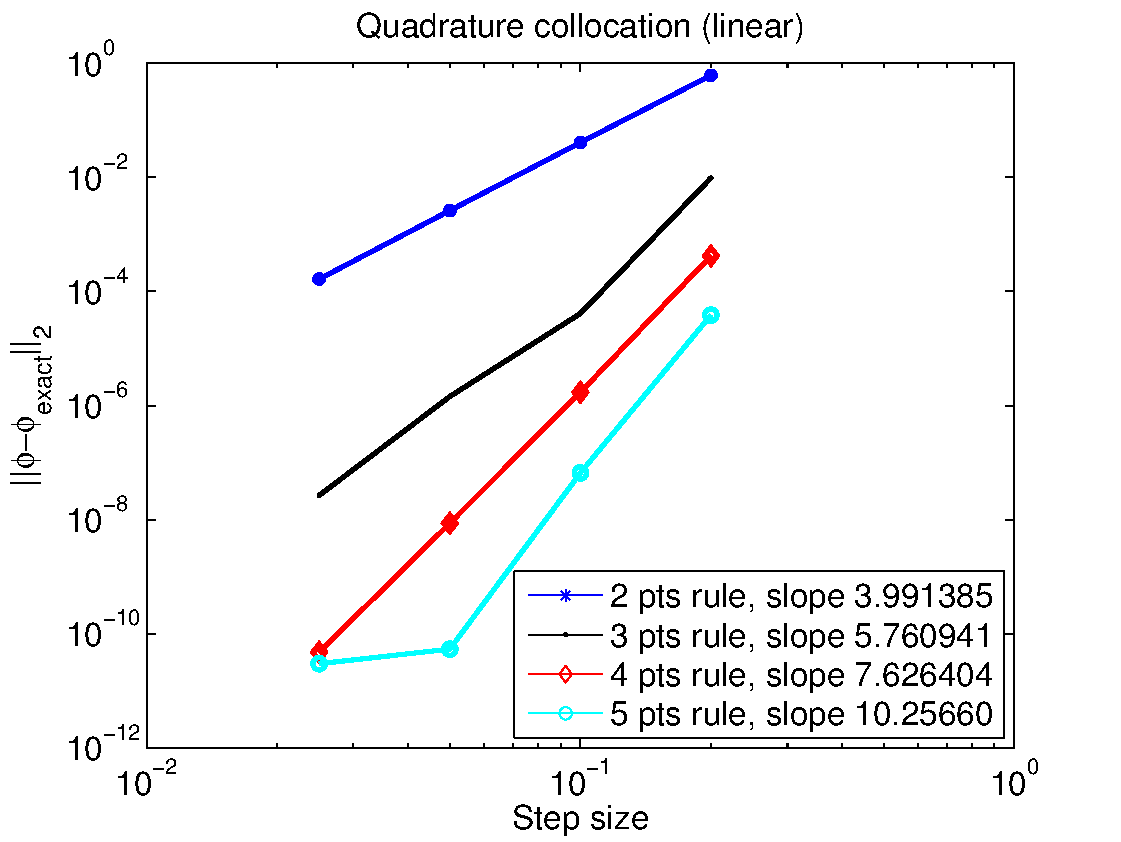
\includegraphics[height=1.7in]{error-norm-qc}
\caption{Convergence of propagator accuracy with respect to time step.}
\label{F:errWAVE}
\end{figure}

To demonstrate the order of accuracy, we plot the wave function error
(in terms of the 2-norm) against step size in \figurename~\ref{F:errWAVE}.
The error of the exponential propagators converges as expected: $O(dt^N)$ for time steps $dt$ with method of order N.
Similarly, the error of the QCM with $n$ quadrature points displays a numerical accuracy: $O(dt^{2n})$
The plateau of the 5-pt QCM in \figurename~\ref{F:errWAVE}-right
comes from the spatial truncation error.
For a given time step, the errors produced by the QCM are about 100 times less than
those of the exponential propagator.
Thus, the QCM outperform the exponential operators in the linear problem.

To further explore the convergence of our propagators, we examine errors in energy and wave function norm
in \figurename~\ref{F:errEN_WAVE}. We see that Chin-Chen (CC), representative of the exponential propagators)
is more accurate than the QCM2 (QCM with 2 quadrature points) for a given step sizes.
\begin{figure}[hbt]
\centering
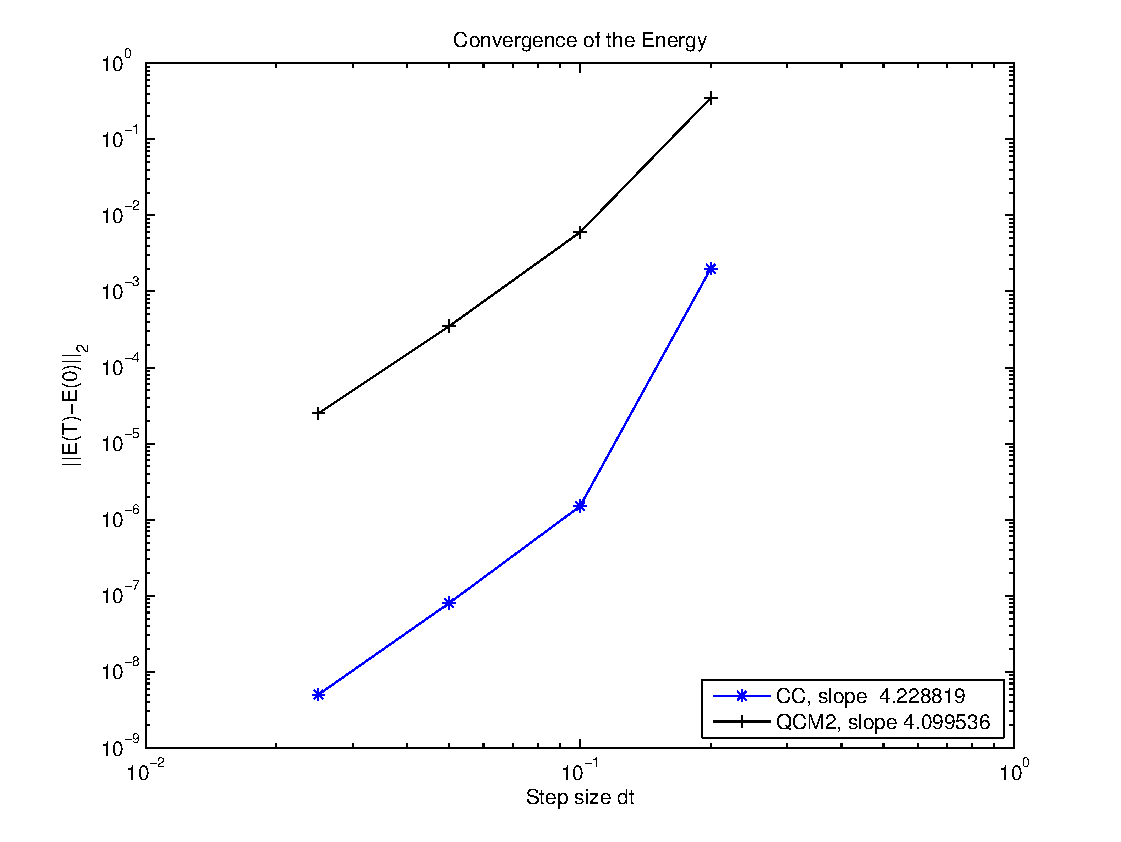
\includegraphics[width=2.35in,height=2.2in]{energy-norms}
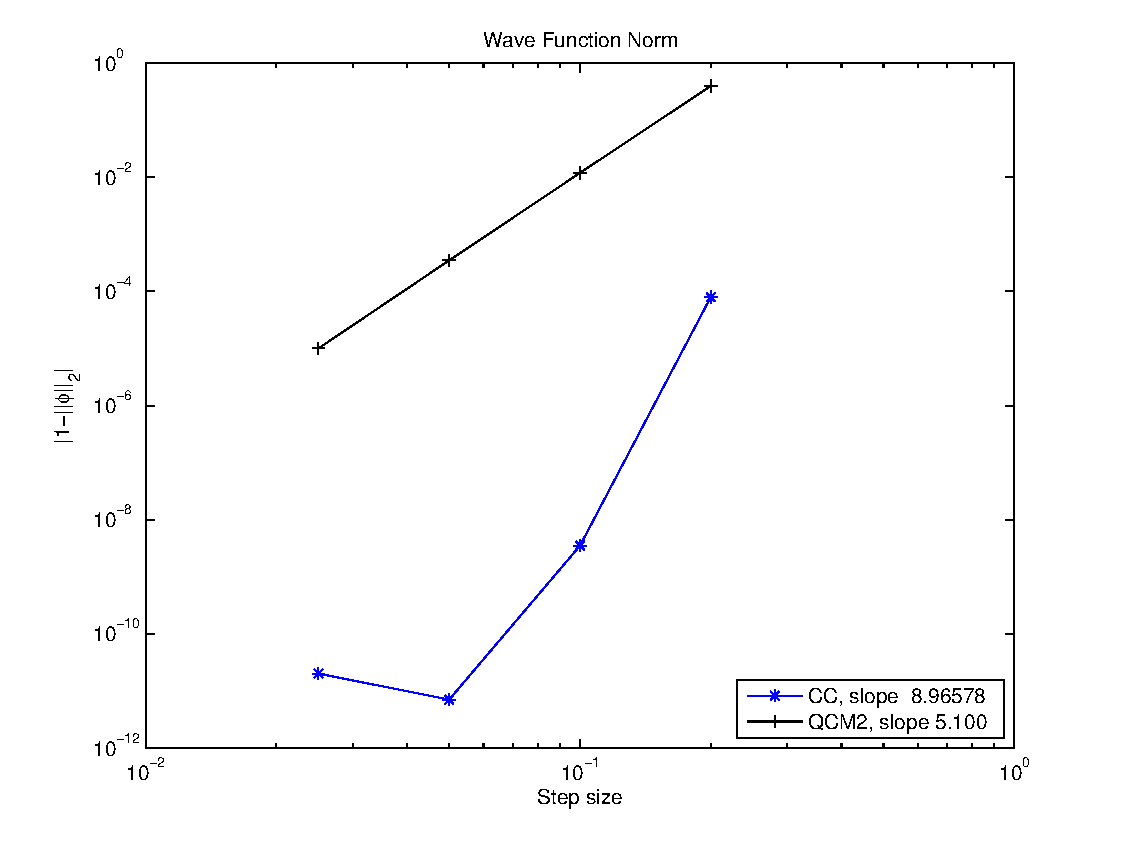
\includegraphics[width=2.35in,height=2.2in]{norms}
\caption{Convergence of the energy and norm for Chin-Chen (CC) and QCM2.}
\label{F:errEN_WAVE}
\end{figure}
Interestingly, QCM2 does not conserve wave function norm,
for the error in wave function norm (see Fig. \ref{F:errEN_WAVE})
\begin{equation}
\varepsilon_{norm} = |1 - \langle \phi \mid \phi \rangle^{1/2}|
\end{equation}
to be an order of magnitude greater than the error in
the wave function (see \figurename~\ref{F:errWAVE}) in terms of 2-norm
\begin{equation}
\varepsilon_{\phi} = ||\phi_{exact}-\phi||_2.
\end{equation}

Despite the norm-preserving construction of the exponential propagators,
these numerical results indicate that, for large step size, norm is not conserved.
This is due to a filtration in the application of free-space propagator
[described in Eq. \eqref{E:matElem}]; we correct for this loss of norm
(via renormalization) when computing expectation values.


\begin{figure}[htbp]
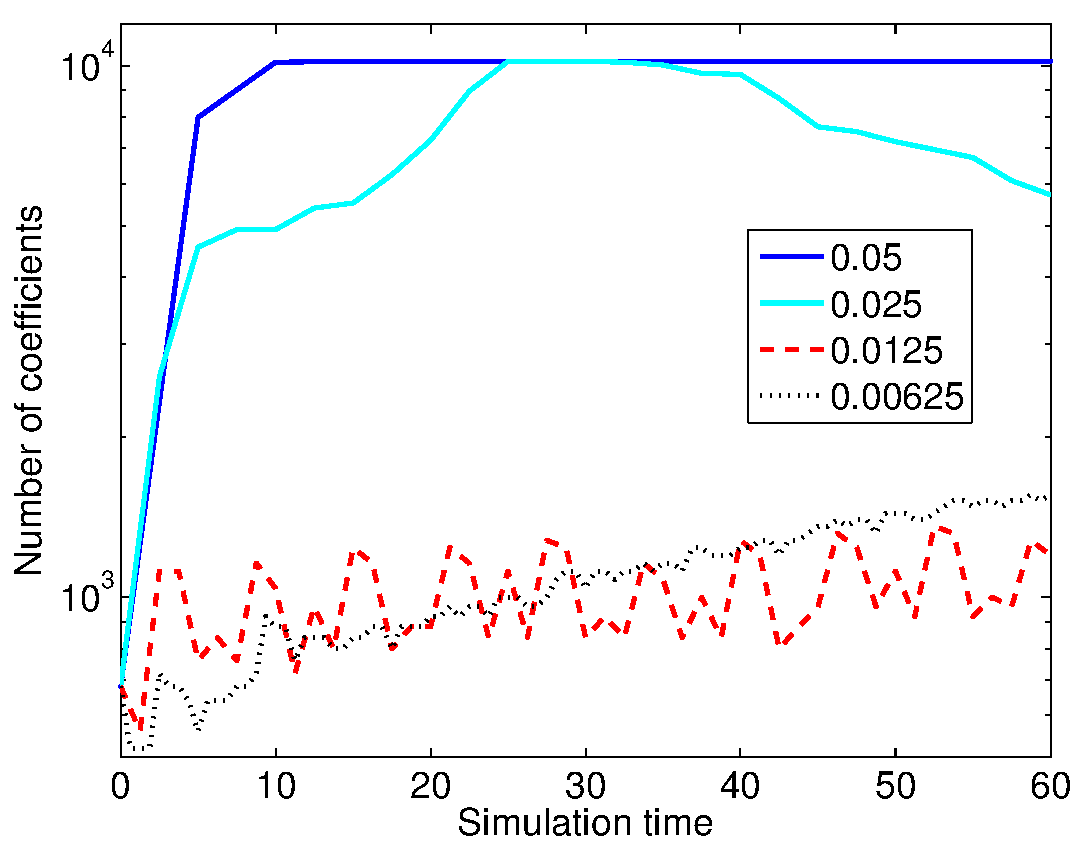
\includegraphics[height=2in]{ncoeff1}
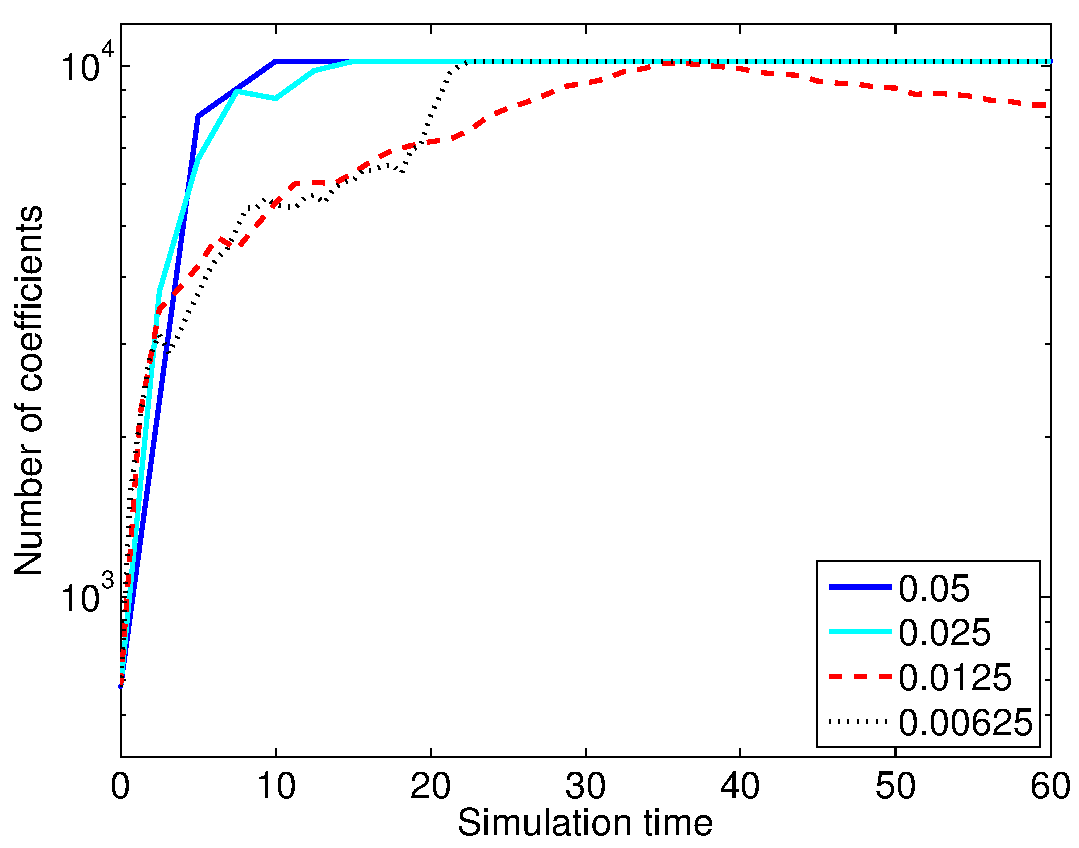
\includegraphics[width=2.35in,height=2.0in]{ncoeff2}
\caption{
Comparing the number of coefficients over time in the QCM and Exponential
propagation schemes for four different time-steps.
}
\label{F:errEnNorm}
\end{figure}


\subsection{Optimization: size and depth}
We now examine several factors involved in choosing an optimal propagator.
In MADNESS, an ideal propagator would maintain a constant number
of coefficients throughout the translation of a wave function.
\figurename~\ref{F:errEnNorm} shows the number of coefficients for the exponential
propagators increasing with time, while the higher order  QCM keeps this number small indicating that QCM
quench numerical noise better. \figurename~\ref{seq:refFig.11} shows that the depth of
adaptive refinement is preserved throughout the simulation.
Since the purpose of adaptivity is maintaining accuracy with a sparse representation;
this ability to preserve structure adaptively is a key to efficiency -- especially
in accurate, high-dimension simulations.

While the QCM quench noise by minimizing the number
of coefficients throughout time propagation, the exponential
propagators are more efficient in the number of operator applications per time
step (see \tablename~\ref{seq:refTable0}).
Fig. \ref{F:accu4} \& \ref{F:accu13} compare them at different truncation threshold.
For a spatial truncation threshold of $\epsilon=10^{-4}$, the Chin-Chen propagator
fails to reduce the error in  \figurename~\ref{F:accu4} with decreasing step sizes, while the QCM
produces an additional digit of accuracy with $dt=0.025$.
For a spatial truncation threshold of $\epsilon=10^{-13}$, the Chin-Chen propagator outperforms
the QCM in \figurename~\ref{F:accu13} reducing the final propagation error as $dt$ decreases.
However, since we are interested in efficient application over longer time steps,
we chose Chin-Chen for the 3D simulation \cite{Vence:2012iy} in Section \ref{S:hatom}.

\begin{table}[htbp]
\caption{
 Propagator complexity in terms of:
 $N$ - Number of free-space propagator applications per time step; and $m$ -
 the number of fixed point iterations used to solve Equation~\eqref{qcform}.
 }
\label{seq:refTable0}
\begin{supertabular}{|m{0.78in}|m{0.5in}|m{0.5in}|m{0.5in}|m{0.5in}|m{0.6in}|}
\hline
- & Trotter & CC & FG4 & FG6 &  $n$ pts rule \\
 \hline
$N$ & 2 & 2 & 2 & 3 & $m \times n^2+n$\\
\hline
\end{supertabular}
\end{table}


\begin{figure}[htbp]
\centering
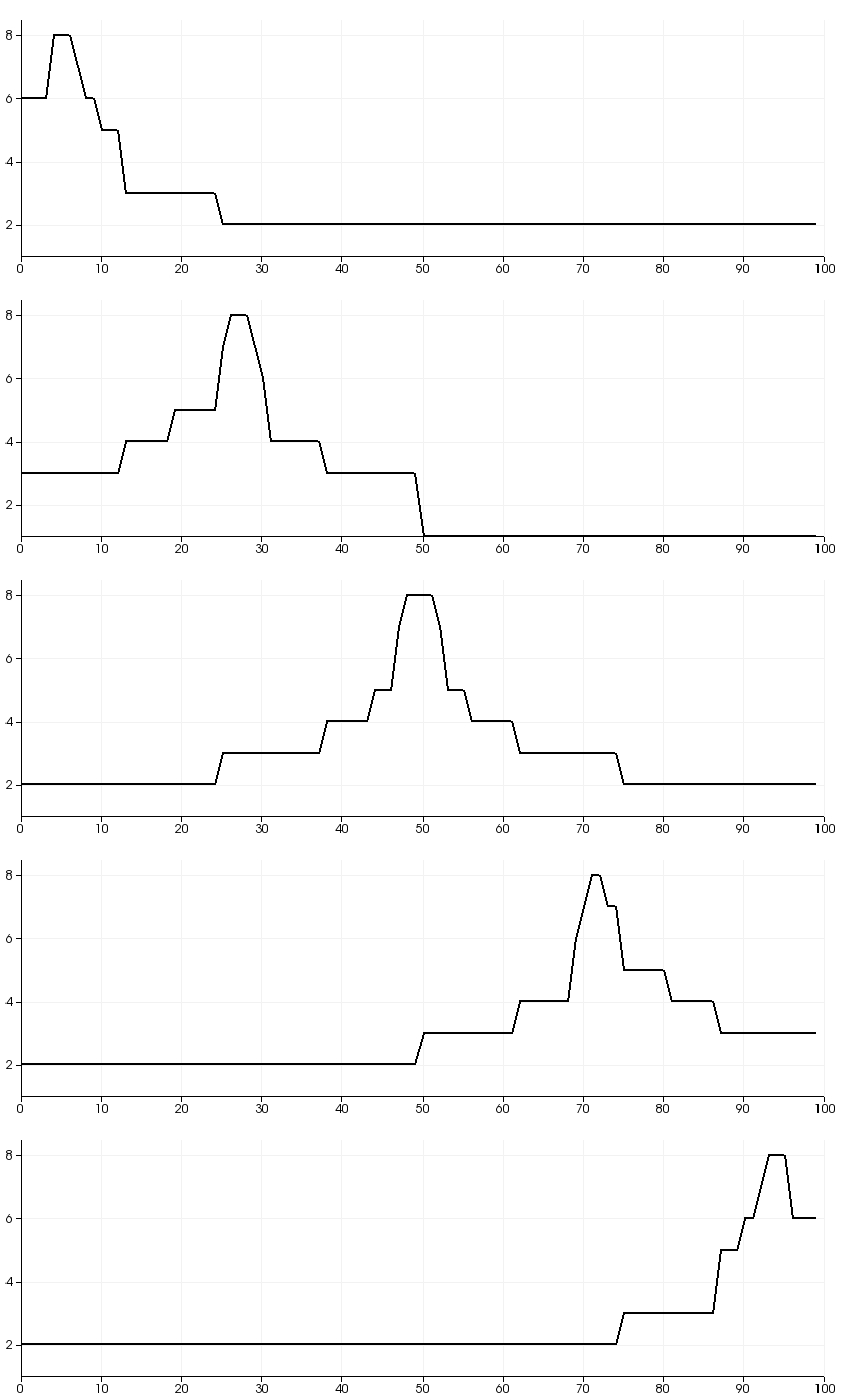
\includegraphics[width=1.8in]{depth.jpg}
\caption{For the linear TDSE (see Section~\ref{S:linearTDSE}),
the refinement level \emph{vs} distance is plotted at different time steps.
For each higher level, the local grid size is halved. The snapshots were taken at $t=5,27.5,50,72.5,95$ (atomic units).}
\label{seq:refFig.11}
\end{figure}



\subsection{The non-linear TDSE}
These propagators are applied to the non-linear TDSE described in Section~\ref{S:nonLinearTDSE}.
The exponential propagators required extrapolation before they could be applied
to the non-linear problem; however, the fixed-point iteration used by the QCM were
immediately applicable to nonlinear problems.
The convergence behavior of the nonlinear system was very similar to that of linear system, and
we do not reproduce it.


\begin{figure}[ht]
\centering
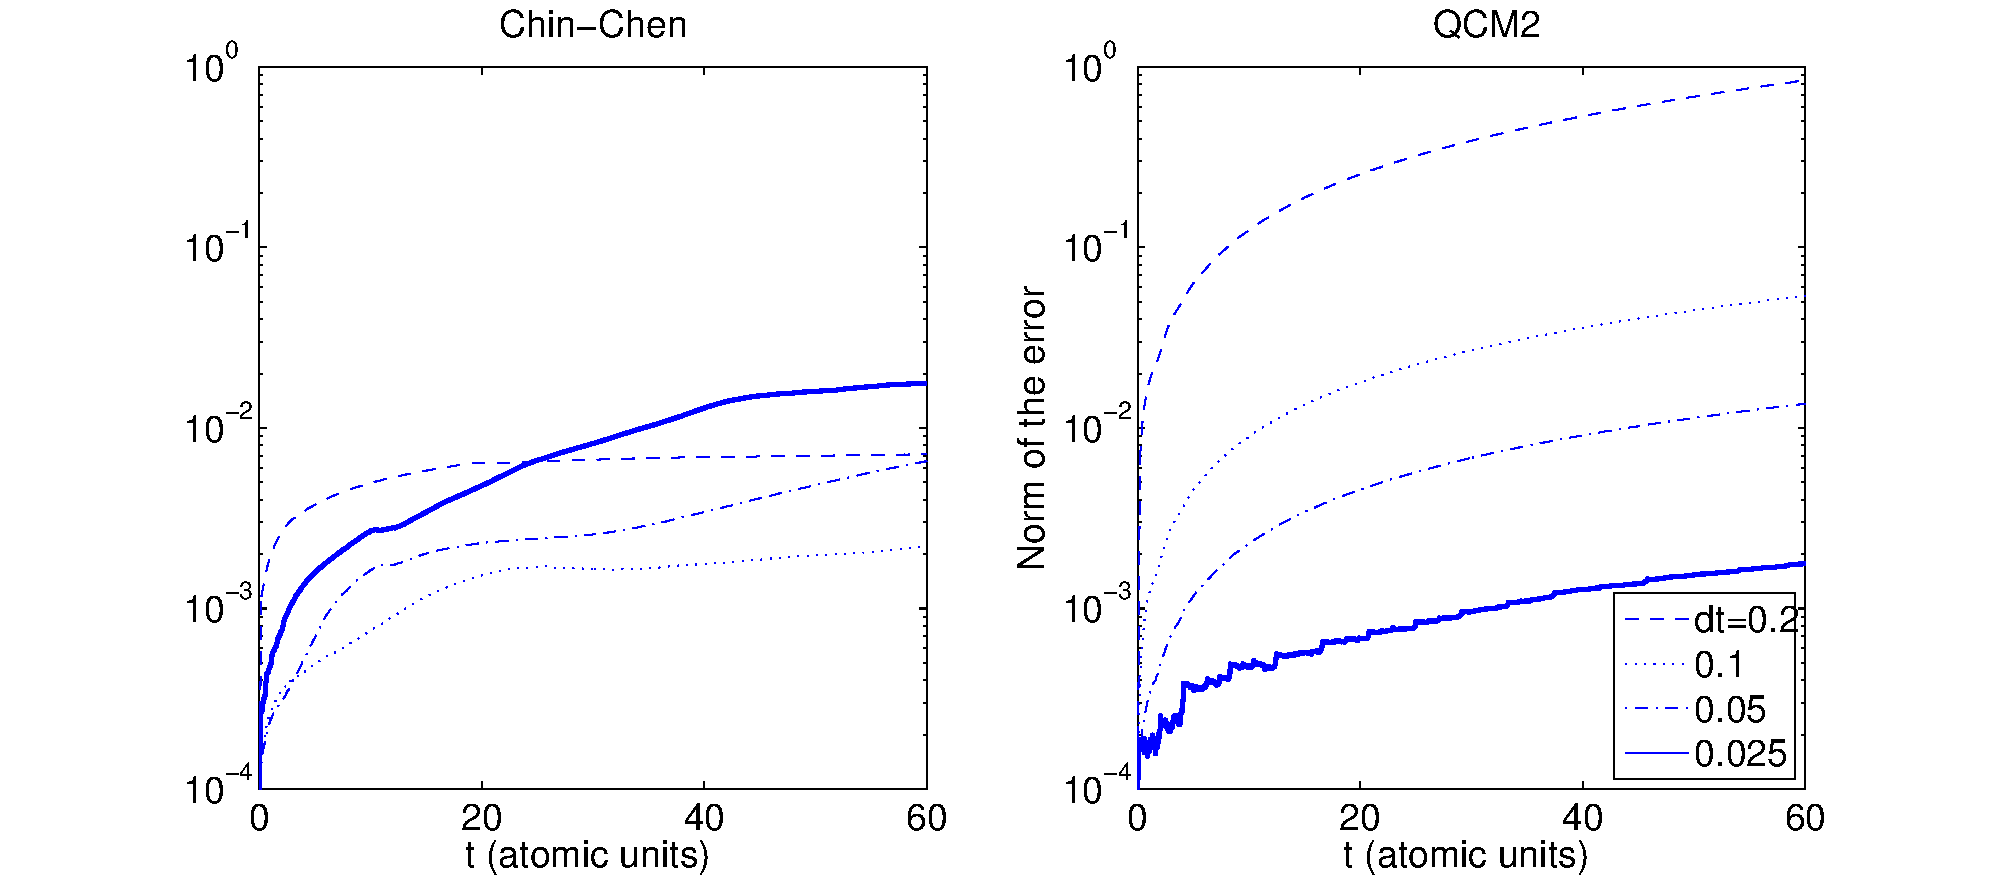
\includegraphics[width=5in]{error_accu4}
\caption{ Error \emph{vs} time is shown for Chin-Chen and QCM2 with a spatial accuracy of $\epsilon~=~10^{-4}$. }
\label{F:accu4}
\end{figure}

\begin{figure}[htbp]
\centering
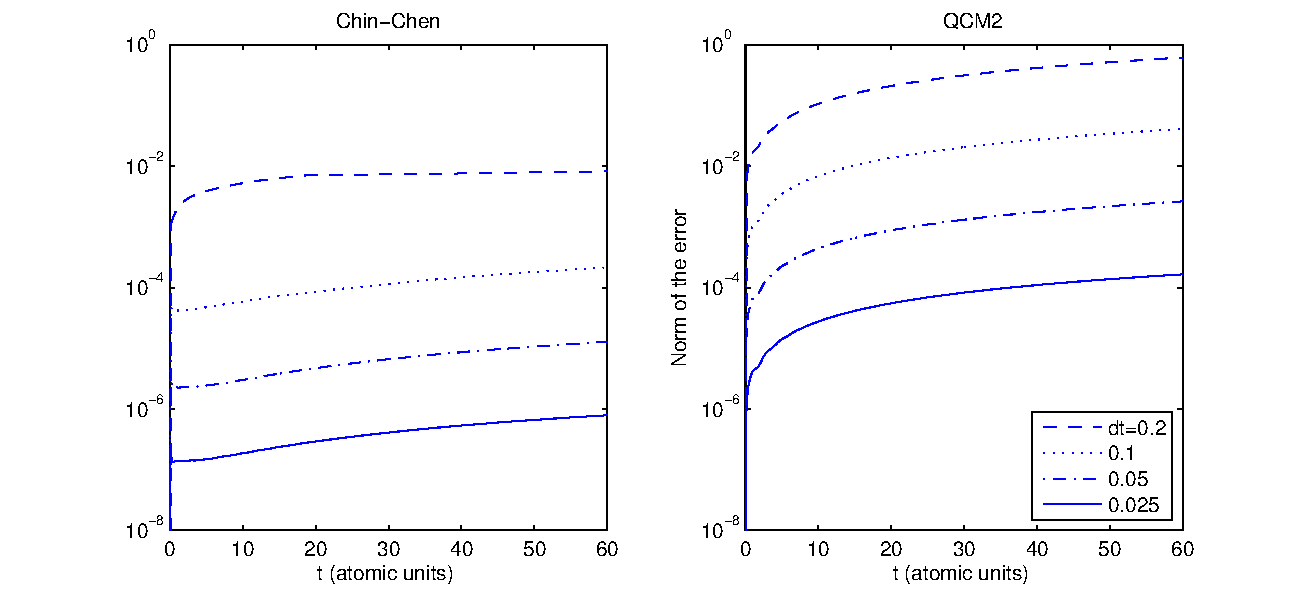
\includegraphics[width=5in]{error_accu13}
\caption{ Error \emph{vs} time is shown for Chin-Chen and QCM2 with a spatial accuracy of $\epsilon~=~10^{-13}$. }
\label{F:accu13}
\end{figure}




\section{Application}
\label{S:hatom}
These propagators are used by physicists interested in the
effects of non-perturbative, few-cycle, laser pulses on atoms/molecules \cite{Krausz:2009hz,Lin:2010cg}
and lightwave engineers developing shorter laser pulses and better measurment technology
\cite{Popmintchev:2010di}. Previously \cite{Vence:2012iy}, we solved the TDSE for hydrogenic atoms
subjected to a strong, attosecond, laser field and calculated the differential photoionization probabilities
along with other observables. \comment{Section \ref{S:AMOmethod} outlines the theoretical approximations ivolved
in our method and Section \ref{S:convdt} discusses the implementation and convergence of time evolution.}


%\subsection{Method}
\label{S:AMOmethod}
The electron behavior is modeled by a three dimensional (3D) wave function beginning in the
ground state and governed by the TDSE within the dipole approximation of the length gauge
\begin{equation}
\label{E:hamiltonian}
i\frac{d\Psi }{dt} =\hat{H}\Psi    \quad\quad\quad
\hat{H} =-\frac{1}{2}\nabla ^{2}+V(r)+\mathbf{E}(t)\cdot \mathbf{r}
\end{equation}
\begin{equation}
\mathbf{E}(t) = E_0 \sin\big(\frac{\omega t}{2 n_{cy}}\big)^2 \sin(\omega t) \notag
\end{equation}
where $\mathbf{E}(t)$ is the electric field strength and $V(r)$ is the atomic potential.

To control high frequencies above the band limit of the propagator, we use a band-limited potential
\begin{align}
V_{model}(r) &=\frac{\text{erf}(r)}{r}+\frac{e^{-r^{2}}}{\sqrt{\pi }}  \\
V_\xi(r)     &= \frac{Z}{\xi }V_{model}(\frac{r}{\xi }) \notag
\end{align}
that converges to the Coulomb potential:
\begin{equation}
\label{E:modelV}
\lim_{\xi \rightarrow 0}V_{\xi }(r) =-\frac{Z}{r}.
\end{equation}
This model potential allows us to propagate exactly within the band limit.
Since it is desirable to begin in an eigenstate of the Hamiltonian, the ground state, Coulomb, wave function
$\displaystyle{\psi(r) = \frac{e^{-r}}{\sqrt{\pi}}}$ was evolved in imaginary time to produce a
numerical eigenstate of the model potential in Eq.~\ref{E:modelV}.
Time propagation is then accomplished by a repeated application of the Chin-Chen propagator.

%\subsection{Convergence}
\label{S:convdt}

\begin{figure}[tbhp]
\begin{center}
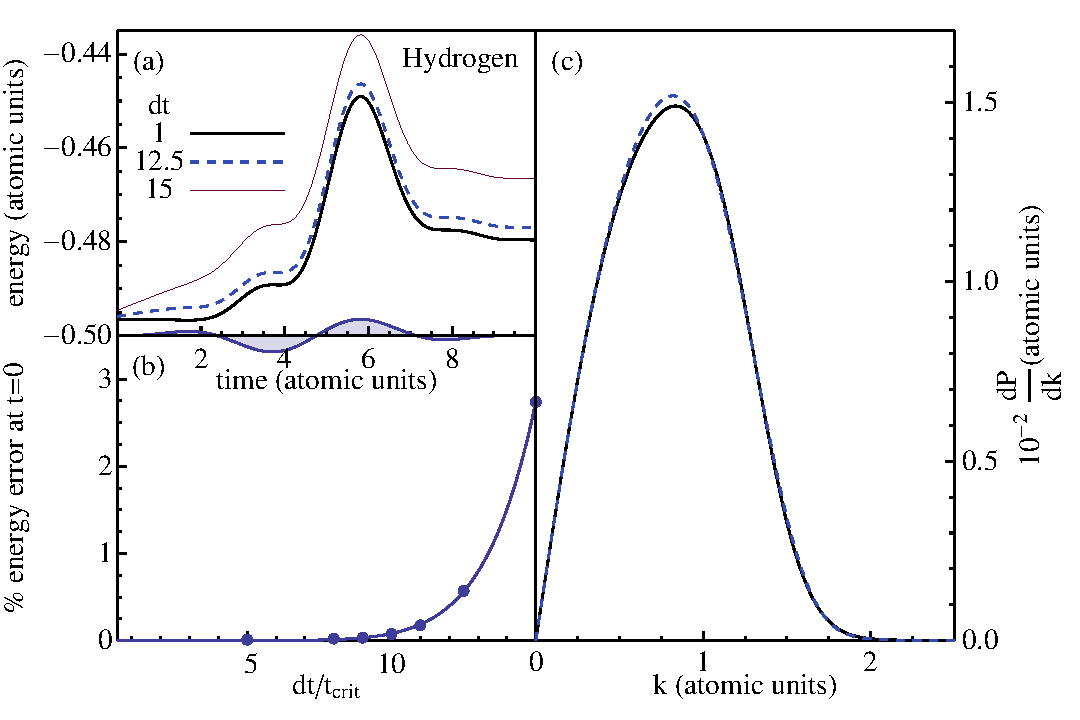
\includegraphics[width=4in]{tSclConv}
\end{center}
\caption{
The convergence of atomic hydrogen
($t_{crit} = 3.4\e{-3}, \xi = 0.2, \epsilon=10^{-5}$) with respect to the time step ($dt$):
(a) the energy $\langle \hat{H} \rangle$ as a function of time,
(b) the error (compared with $dt = t_{crit}$) of final energy for various $dt$, and
(c) the photoionization spectrum for various $dt$.
}
\label{F:tScale}
\end{figure}

Time step optimization seeks to maximize the efficiency and minimize error.
At each time step ($dt$), error is accumulated from the size of the time step
($\varepsilon_{dt}$) and the truncation ($\varepsilon_{trunc}$) of the adaptive basis.
\begin{equation}
\varepsilon_{total} = O\big(\frac{T \varepsilon_{trunc}}{dt}\big)
                    + O\big(\frac{T \varepsilon_{dt}}{dt}\big)
\end{equation}
While $\varepsilon_{dt}$ dominates at large time steps, $\varepsilon_{trunc}$
becomes a factor with small $dt$ (many time steps).
Fig.~\ref{F:tScale}(a) shows how step size affects the
energy (expectation value of the Hamiltonian) of hydrogen \emph{vs} time.
Note the following numerical artifacts. First, the ground state energy
[at $t=0$ in Fig.~\ref{F:tScale}(a)] is larger than its true value of -0.5; this
comes from a finite value of $\xi$ and it converges to -0.5 as $\xi \rightarrow 0$.
Second, notice the slight elevation of $dt=12.5$ at the end of the pulse in Fig.~\ref{F:tScale}(a)];
Fig.~\ref{F:tScale}(b) plots this relative error as a function of $dt$.
That no appreciable error is present before $dt = 10 t_{crit}$ showcases the efficacy of the large time
steps enabled by the high-order, symplectic integrator \cite{Chin:2001vs} [from Eq. \ref{E:CC}].
This error quickly diverges with increasing dt.
Finally, photoionization [see Fig.~\ref{F:tScale}(c)] is largely insensitive to $dt$.


\section{Conclusions}
We have studied various propagators for the time-dependent Schro\"odinger equation in an adaptive,
discontinuous, multi-wavelet basis. After reviewing the methodology of our band limited propagator,
we demonstrated its effectiveness time evolving a complex Gaussian. After reviewing
the exponential and quadrature-collocation propagators, we used the translating-atom test-problem
as a metric for comparison.
After analyzing the discrepancies in the energy and norm over various time steps, we
decided that Chin-Chen was the ideal propagator for our numerical scheme.
Finally, we applied the Chin-Chen propagator on a 3D, \emph{ab initio} treatment of atomic
hydrogen in a strong laser field.

\section{Acknowledgments}
This material is based upon work supported by the National Science Foundation under Grant No. OCI-0904972 to RJH.
This research is sponsored by the Office of Advanced Scientific Computing Research (OASCR); U.S. Department of Energy. The work was performed at the Oak Ridge National Laboratory, which is managed by UT-Battelle, LLC under Contract No. DE-AC05-00OR22725.
GF is support in part by the OASCR's Math base program; GF and JJ were supported in part by OASCR's EASI! Math/CS Institute Project.
This research used resources of the Oak Ridge Leadership Computing Facility at Oak Ridge National Laboratory, which is supported by the Office of Science of the Department of Energy under Contract No. De-AC05-00OR22725.

\bibliographystyle{plain}
\bibliography{qmprop,common}

\end{document}
